\documentclass[../main.tex]{subfiles}

\begin{document}
	\begin{figure} [h]
		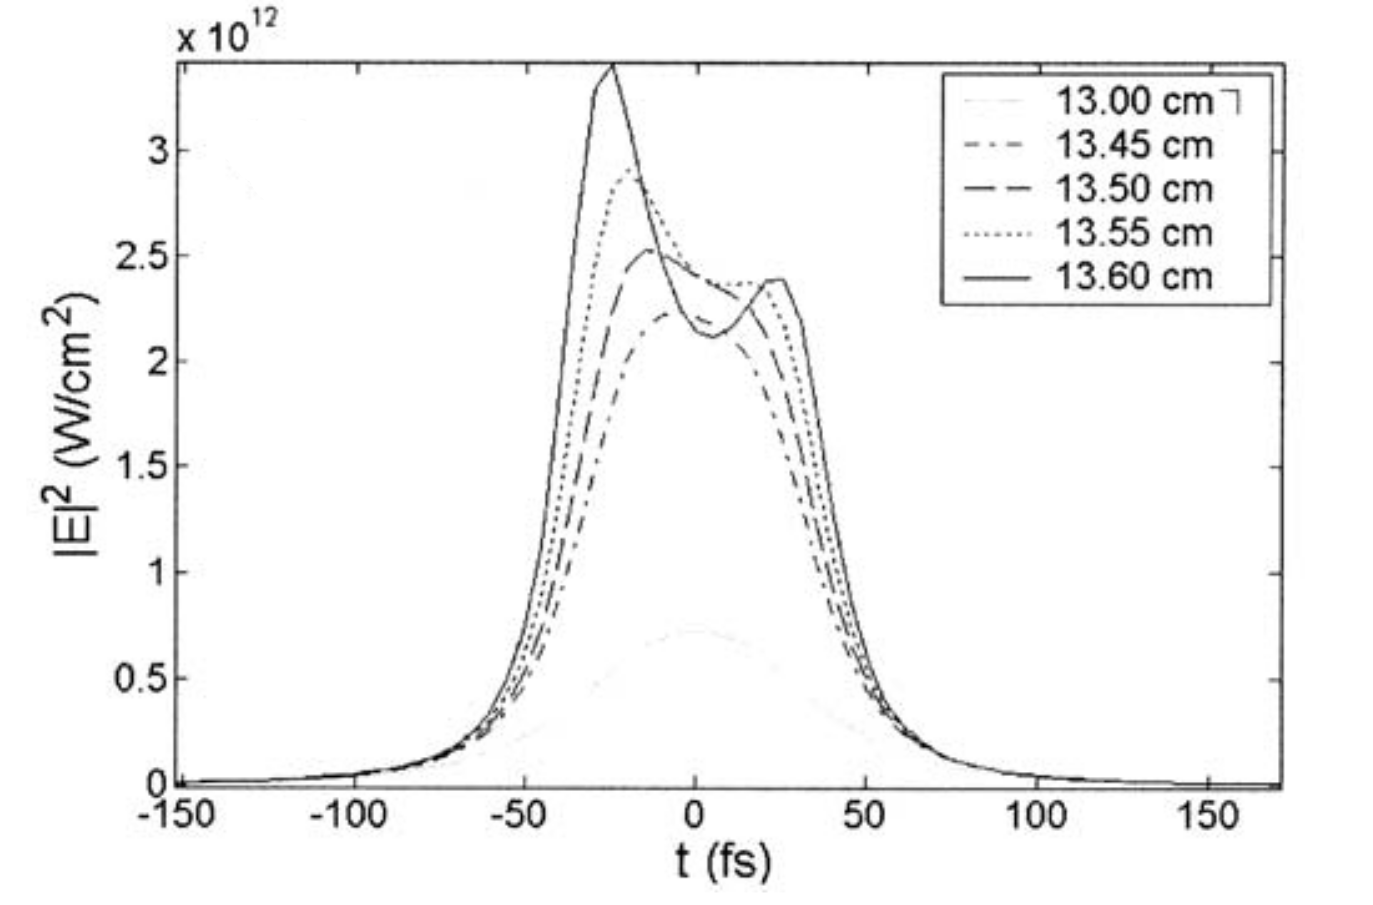
\includegraphics[width=0.5\textwidth]{images/split_ion.png}
		\caption{Temporal splitting at nonlinear focus for $5P_{cr}$.
		\label{fig:split_ion}}
	\end{figure}

	\begin{figure} [h]
		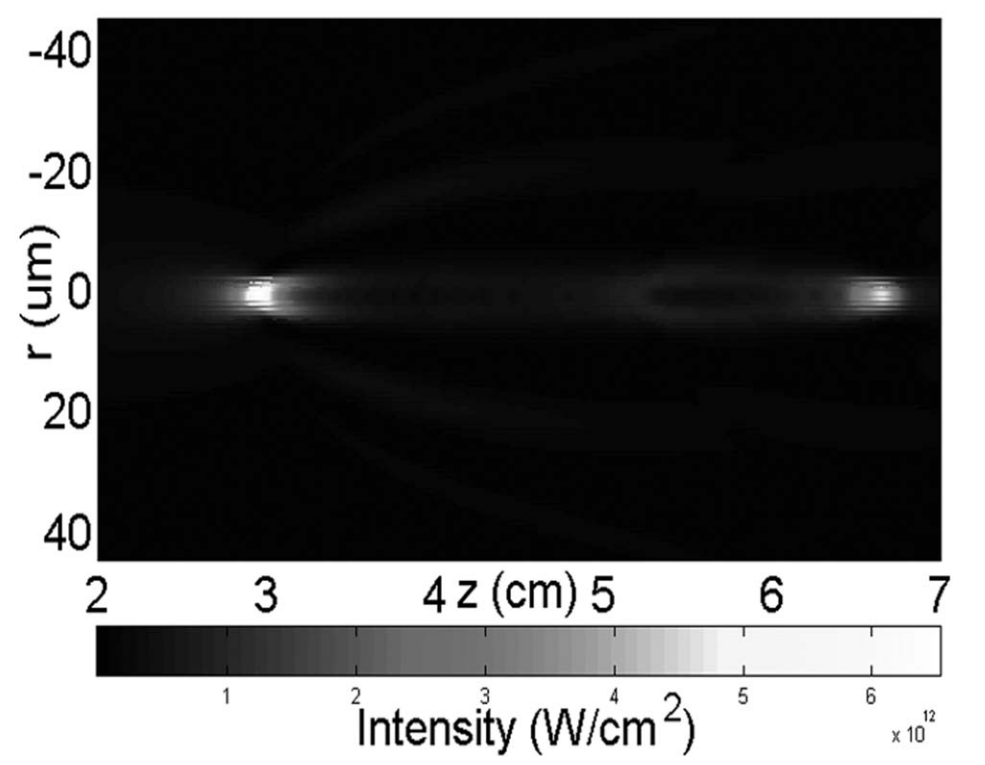
\includegraphics[width=0.5\textwidth]{images/filament1.png}
		\caption{On-axis defocusing - focusing cycle in ionization
			regime.
		\label{fig:fila_ion}}
	\end{figure}

	When input power of pulse is more than $P_{th}$, then we enters ionization
	regime. If we take notice of fig [\ref{fig:char_len}], for power more
	than $P_{th}$, $z_{sf}$ is smaller than $z_{nlgvd}$. Therefore collapse
	due to self focusing can not be prevented by GVD alone.
	These larger intensities enable nonlinear photoionization and
	generate plasma in our medium, and defocusing due to plasma came into
	play.
	In this regime, flaments are formed which propagate over several of
	Rayleigh lengths without divergence. In air, these distances could be
	upto several kilometres.


	\paragraph{\textbf{Asymmetric pulse splitting}}
	When this intense pulse moves through medium, leading part of pulse
	creates plasma with being much effected by it. The trailing part is
	defocused by that plasma which was generated by leading edge. Because
	both the edge interact differently with the medium, we see a asymmetric
	pulse splitting. See figure [\ref{fig:split_ion}].
	The trailing edge is lower in intensity because it get defocused due to
	plasma, while leading edge pass nearly unaffected. It changes form of
	pulse from being single peaked to a two peaked pulse with unequal peaks.
	The on-axis splitting takes placed due to plasma defocusing and we have
	a spatial ring profile. Now on axis, there is not enough intensity for
	plasma creation. Therefore both peaks start to self focus and get split.
	Then this cycle of focusing-defocusing continues till different flaments
	of beam have less peak power tha $P_{cr}$. See figure
	[\ref{fig:fila_ion}].
\end{document}
